\section{Solution using SVD}
\label{sec:ls:SVD}
The \asvd \ is a powerful theoretical tool for studying the least squares problem. In addition to needing the decomposition products, we will need to exploit the unitary equivalence of the $2-$norm, the norm of least squares.

%%%%%%%%
\subsection{Unitary transformation}
The gift of unitary transformation allows us to take a difficult problem and convert into a more benign form. 

%%%%%%%%
%%%%%%%%
\subsubsection{Invariance of the $2-$norm}
The importance of this class of transformations commands review. The $2-$norm\footnote{This is also true for the Frobenius norm.} is preserved under unitary transformation. Let $\A{}$ be the obligatory rectangular matrix in $\cmplxmn$ and consider the unitary matrices $\WW{} \in \cmplxmm$ and $\Z{} \in \cmplxnn$. The invariance of the $2-$norm is expressed by 
\begin{equation}
\begin{split}
  \normt{ \WW{} \A{} } &= \normt{ \A{} }, \\
  \normt{ \A{}\,\Z{} } &= \normt{ \A{} }.
\end{split}
\end{equation}

The proof is painless. Start with the first case and use a definition for norm as the greatest dilation of vectors composing the unit ball:
\begin{equation}
  \normts{ \WW{} \A{} } = \mxball \normts{ \WW{} \A{} x }.
\end{equation}
Express the norm as an inner product:
\begin{equation}
  \normts{ \WW{} \A{} x } 
    = \paren{\WW{} \A{} x}^{*} \paren{\WW{} \A{} x} 
\end{equation}
In this form we can exploit the defining property of the unitary matrix:
\begin{equation}
  \WW{*}\WW{} = \I{m}
\end{equation}
because
\begin{equation}
  \paren{\WW{} \A{} x}^{*} \paren{\WW{} \A{} x} 
    = x^{*}\A{*}\paren{\WW{*}\WW{}} \A{}x
    = \paren{x^{*}\A{*}}  \paren{\A{}x}.
\end{equation}
Now we go back to the norm structure
\begin{equation}
  \paren{x^{*}\A{*}}  \paren{\A{}x} = \normts{ \A{} x }
\end{equation}
This demonstrates
\begin{equation}
  \normts{ \WW{} \A{} } 
    = \mxball \normts{ \WW{} \A{} x }
    = \mxball \normts{ \A{} x } 
    = \normts{ \A{} } .
\end{equation}
Because the norm is positive definite we can take the positive value for the square root and state
\begin{equation}
  \normt{ \WW{} \A{} } = \normt{ \A{} }.
\end{equation}

To show the other equality
\begin{equation}
  \normt{ \AZ } = \normt{ \A{} }
\end{equation}
the insight is to exploit the fact that
\begin{equation}
  \normt{ \A{*} } = \normt{ \A{} }
\end{equation}
and work with the adjoint matrix $\paren{\AZ}^{*} $.

We have seen invariance of the $2-$norm under unitary transformation of a matrix by premultiplication and by posmultiplication. This implies invariance under simultaneous transformation:
\begin{equation}
  \normt{ \WW{} \AZ } = \normt{ \WW{} \paren{\AZ}  } = \normt{ \AZ } = \normt{ \A{} }.
\end{equation}


%%%%%%%%
%%%%%%%%
\subsubsection{Transforming the least squares problem}
For the overdetermined problem there is no \ns \ $\rnlla{}$ for the domain. If $m=n$, then the there is no \ns \ $\rnlla{*}$ for the codomain either. When $m > n$, the first $n$ columns of $\V{}$ span $\brnga{}$, the last $n-m$ columns span the  \ns \ $\rnlla{*}$. The structure of the decomposition for the overdetermined system is this
\begin{equation}
  \A{} = \csvdblockb{*} 
\end{equation}
We use a unitary matrix to transform the problem into a simpler form
\begin{equation}
  \begin{split} 
    \minimum 
      &= \normts{ \U{*} \paren{ \A{} x - b }  }.
  \end{split} 
\end{equation}
Now we can apply the \asvd in this form
\begin{equation}
  \U{*} \A{} = \sig{} \, \V{*}.
\end{equation}
The least squares problem becomes
\begin{equation}
  \begin{split} 
    \minimum 
      = \normts{ \sig{} \, \V{*} x - \U{*} b }
      &= \normts{ \sbb{} \, \bvr{*} x - \cublockfs{*} b } \\
	    &= \normts{ \mat{c}{ \ess{} \bvr{*} x \\[3pt]\hline\zero  } - \mat{c}{ \bur{*} b \\[3pt]\hline \run{*} b } }
  \end{split} 
\end{equation}
We have now untangled the range space components from the \ns \ components.


%%%%%%%%
\subsection{The SVD solution for least squares}
We rely upon the Pythagorean theorem\index{Pythagorean theorem} to isolate the range and \ns \ components of the total error for the least squares problem
\begin{equation}
  \minimum = \underbrace{\normts{ \ess{} \bvr{*} x -\bur{*} b  }}_{x \text{ dependence}} + \underbrace{\normts{ \run{*} b  }}_{\text{residual}}
\end{equation}
There are now two terms; the first depends upon the solution vector $x$, the second does not. We only have control over the first term. To minimize the total error we must drive the first term to zero. Then the total error will be given by the residual error\index{least squares!residual error!\ns\ terms} term.
The error term that is controlled by the solution vector $x$ is this
\begin{equation}
  \ess{} \bvr{*} x - \bur{*} b .
\end{equation}
We choose $x$ to force this term to zero. This leads to the SVD solution\index{least squares!solution!SVD} for the least squares problem:
\begin{equation}
  \xmp = \bvr{} \ess{-1} \bur{*} b.
  \label{eq:svd soln}
\end{equation}
This is the pseudoinverse solution\index{least squares!solution!pseudoinverse}
\begin{equation}
  \xmp = \Ap b
\end{equation}
where the (thin) pseudoinverse is
\begin{equation}
  \Ap = \bvr{} \ess{-1} \bur{*}.
  \label{eq:mpptsvd}
\end{equation}

It is always a good idea to verify conformability by writing out the matrix dimensions and table \eqref{tab:least squares:svd dims} shows the dimension of the matrices and vectors in the pseudoinverse solution
%%
\begin{table}[!htdp]
%\caption[Dimensions of the decomposition]{default}
\begin{center}
\begin{tabular}{cccccc}
%
  $x$ & $=$ & $\bvr{}$ &  $\ess{-1}$  & $\bur{*}$ & $b$ \\
%
  $\by{n}{1}$ & $=$ & $n\times \rho$ & $\rho\times \rho$ & $\rho\times m$ & $m\times 1$
%
\end{tabular}
\end{center}
\label{tab:least squares:svd dims}
\end{table} \\
%%
What we shown is that the vector $x$ which minimizes the least squares error in \eqref{eq:lsmin} is exactly the same vector given by the SVD solution in equation \eqref{eq:svd soln}. Using a unitary transform we were able to convert the general least squares problem into a form amenable to solution using the \asvd.

For the overdetermined case as we have here the usually silent \ns \ term can be heard as it pronounces the value of the total error
\begin{equation}
  r^{2} = \normts{ \run{*} b  } = \paren{ \run{*} b  }^{*} \paren{ \run{*} b  } = b^{*} \paren{ \run{}\run{*} } b 
  \label{eq:r2:a}
\end{equation}


%%%%%%%%
\subsection{Example}
Consider the linear system
\begin{equation}
  \begin{split}
    \axaeb, \\
    \matrixb \xtwo &= \datab.
  \end{split}
\end{equation}
The pseudoinverse is shown in equation \eqref{eq:mpptsvd} allowing us to compute the particular solution as
\begin{equation}
  \bxls = \Ap b = \Aplusb \datab = \xlsb.
\end{equation}
Since the matrix $\A{}$ has full column rank the \ns \ $\rnlla{}$ is trivial and there is no contribution from an inhomogeneous solution. Therefore we must have
\begin{equation}
  \bxls \in \brnga{*}.
\end{equation}


The residual error vector is given by
\begin{equation}
  {\rd{ r }} = {\bl{ \axmb }} = \databAxls - \datab = \databr.
\end{equation}
Here is an important point: the method of least squares resolves the data vector into a range space component and a \ns \ component.
\begin{equation}
  \begin{split}
      b\quad\ &= \quad \ \quad  {\bl{ \Ax }} \    \  - \ \qquad \ {\rd{ r }} \\
    \datab &= \underbrace{\databAxls}_{\brnga{}} - \underbrace{\databr}_{\rnlla{*}}
  \end{split}
  \label{eq:least squares:svd:subtract}
\end{equation}
See figure \eqref{fig:least squares:triangle}.
We seen then that the least squares solution subtracts out the \ns \ component in the data vector. While the idea seems basic, it eludes students at times. One way to visualize the leasts squares solution is to express the general solution in terms of a particular solution and a homogeneous solution. The particular solution is expressed in terms of $a_{k}$, $k=\lst{1:\rho}$, the column vectors of the matrix $\A{}$. Clearly, the column vectors are in range $\brnga{}$. The homogenous solution is an arbitrary combination of the columns of $\rvn{}$. Therefore the general solution becomes
\begin{equation}
  \Ax_{LS} = \underbrace{x_{1} {\bl{ a_{1} }} + \dots + x_{\rho} {\bl{ a_{\rho} }}}_{\text{image of solution vector}}\ +\ \underbrace{\alpha_{1} {\rd{ v_{\rho+1} }} + \dots +  \alpha_{n-\rho} {\rd{ v_{n} }}}_{\text{homogeneous solution}}, \quad \alpha \in \cmplx{}.
\end{equation}
The data vector $b$ and the image of the solution vector $\Ax$ are coplanar as shown in figure \eqref{fig:least squares:triangle} below. We will see presently the importance of $\theta$, the angle between them. For example, if the data is in the \ns \ ($\theta = \pi/2$) exclusively then there is no range component and the solution is trivial. 


%
\begin{figure}[htbp] %  figure placement: here, top, bottom, or page
   \centering
   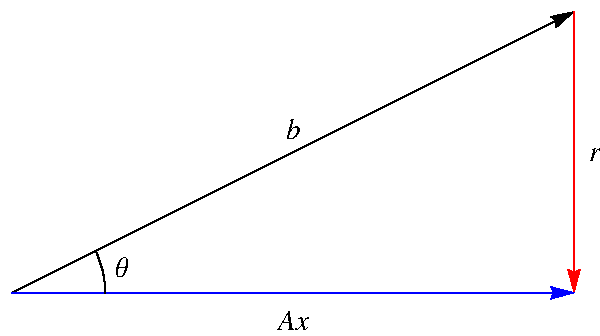
\includegraphics[ width = 3in ]{images/"least squares"/triangle} 
   \caption[The least squares solution is the projection of the data vector into $\brnga{}$]{The least squares solution is the projection of the data vector into $\brnga{}$. The red arrow represents the residual error, the error which cannot be removed. This is a distillation of figure /eqref{fig:least squares:projection}.}
   \label{fig:least squares:triangle}
\end{figure}

Finally, we compute the error. The square of the norm of the residual error vector is the total error:
\begin{equation}
  r^{2} = r^{\mathrm{T}}r = \normbrs.
\end{equation}
This agrees with the method of equation \eqref{eq:r2:a}:
\begin{equation}
\begin{split}
      r^{2} 
       &= \normts{ \run{*} b  } = \paren{ b^{*} \run{} } \paren{ \run{*}  b} \\
       &= \paren{\databt \vecbyna}  \paren{\vecbynat \datab}  \\
       &= \normbrs.
 \end{split}
\end{equation}



\endinput